\documentclass[a4 paper]{article}
% Set target color model to RGB

% Portugues
\usepackage[brazilian]{babel}
\usepackage[utf8]{inputenc}
\usepackage[T1]{fontenc}
\usepackage{bibentry}
\nobibliography*

\usepackage[inner=2.0cm,outer=2.0cm,top=2.5cm,bottom=2.5cm]{geometry}
\usepackage{setspace}
\usepackage[rgb]{xcolor}
\usepackage{verbatim}
\usepackage{subcaption}
\usepackage{amsgen,amsmath,amstext,amsbsy,amsopn,tikz,amssymb,tkz-linknodes}
\usepackage{fancyhdr}
\usepackage[colorlinks=true, urlcolor=blue,  linkcolor=blue, citecolor=blue]{hyperref}
\usepackage[colorinlistoftodos]{todonotes}
\usepackage{rotating}
%\usetikzlibrary{through,backgrounds}
\hypersetup{%
pdfauthor={Ashudeep Singh},%
pdftitle={Homework},%
pdfkeywords={Tikz,latex,bootstrap,uncertaintes},%
pdfcreator={PDFLaTeX},%
pdfproducer={PDFLaTeX},%
}
%\usetikzlibrary{shadows}
% \usepackage[francais]{babel}
\usepackage{booktabs}
\newcommand{\ra}[1]{\renewcommand{\arraystretch}{#1}}

\newtheorem{thm}{Theorem}[section]
\newtheorem{prop}[thm]{Proposition}
\newtheorem{lem}[thm]{Lemma}
\newtheorem{cor}[thm]{Corollary}
\newtheorem{defn}[thm]{Definition}
\newtheorem{rem}[thm]{Remark}
\numberwithin{equation}{section}

\newcommand{\homework}[6]{
   \pagestyle{myheadings}
   \thispagestyle{plain}
   \newpage
   \setcounter{page}{1}
   \noindent
   \begin{center}
   \framebox{
      \vbox{\vspace{2mm}
    \hbox to 6.28in { {\bf GCC153:~Mineração de Dados \hfill {\small (#2)}} }
       \vspace{6mm}
       \hbox to 6.28in { {\Large \hfill #1  \hfill} }
       \vspace{6mm}
       \hbox to 6.28in { {\it Professor: {\rm #3} \hfill {\rm #4} %Name: {\rm #5}, Netid: {\rm #6}
       } }
       %\hbox to 6.28in { {\it TA: #4  \hfill #6}}
      \vspace{2mm}}
   }
   \end{center}
   \markboth{#5 -- #1}{#5 -- #1}
   \vspace*{4mm}
}

\newcommand{\problem}[2]{~\\\fbox{\textbf{Etapa #1}}\hfill (#2\%)\newline\newline}
\newcommand{\subproblem}[1]{~\newline\textbf{(#1)}}
\newcommand{\D}{\mathcal{D}}
\newcommand{\Hy}{\mathcal{H}}
\newcommand{\VS}{\textrm{VS}}
\newcommand{\solution}{~\newline\textbf{\textit{(Solution)}} }

\newcommand{\bbF}{\mathbb{F}}
\newcommand{\bbX}{\mathbb{X}}
\newcommand{\bI}{\mathbf{I}}
\newcommand{\bX}{\mathbf{X}}
\newcommand{\bY}{\mathbf{Y}}
\newcommand{\bepsilon}{\boldsymbol{\epsilon}}
\newcommand{\balpha}{\boldsymbol{\alpha}}
\newcommand{\bbeta}{\boldsymbol{\beta}}
\newcommand{\0}{\mathbf{0}}


\begin{document}
\homework{Orientações para o Projeto da Disciplina}{2019-2}{Eric Fernandes de Mello Araújo}{Versão: \today}{GCC153}{NetId(s)}

\textbf{Instruções importantes}: Leia todas as instruções cuidadosamente antes de começar o seu projeto e antes de submeter no Campus Virtual.
\begin{itemize}
    \item Escreva o projeto em \LaTeX. Use o modelo fornecido neste documento e inclua seu nome e sua matrícula.
    \item Todo o código criado durante a disciplina deve estar em um repositório do Github e referenciado no projeto.
    \item Todas as etapas terão como prazo final para a entrega a meia noite do dia definido, segundo cronograma a seguir.
    \item Entregas fora do prazo acarretarão em redução de 10\% na nota para cada dia de atraso.
    \item Os projetos serão feitos individualmente.
    \item Todas as fontes consultadas deverão ser citadas.
    \item Todos os slides da sua apresentação devem ser enviados pelo Campus Virtual antes do horário de início das apresentações. A não entrega acarretará na perda de 10\% da nota de apresentações. 
    \item Todos os trabalhos serão checados por plágio. Caso existam cópias de textos de outros colegas ou de terceiros, um processo administrativo será instaurado para apurar e punir o estudante que infringir este código de ética.
\end{itemize}

\section*{Descrição}

O desenvolvimento da mineração de dados é reconhecidamente um dos fatores mais relevantes nas alterações das dinâmicas de comportamento no mundo nos últimos anos. O uso de técnicas de extração de informação a partir dos dados causou impactos nas áreas de marketing, política, religião e nas esferas socio-afetivas de nossa sociedade. Os resultados obtidos por meio destas técnicas têm atraído o interesse de empresas e pesquisadores para o quanto se pode aprender sobre os dados de forma automática.

Ao longo do curso, veremos as várias etapas que compõem a mineração de dados, bem como algoritmos e técnicas para este tipo de exploração. A ideia deste projeto é que seja desenvolvido um algoritmo de mineração de dados que passe por todas as etapas do processo, conforme demonstrado na figura \ref{figs:etapas}.

\begin{figure}[htb!]
    \centering
    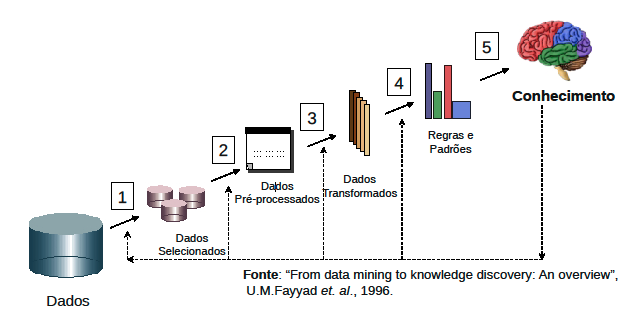
\includegraphics[width=\textwidth]{imgs/etapas_md.png}
    \caption{``From data mining to knowledge discovery: An overview'', U.M.Fayyad et. al., 1996.}
    \label{figs:etapas}
\end{figure}

As seções seguintes apresentarão as etapas do projeto, as instruções, prazos e requerimentos para a avaliação. O projeto é composto de 3 (três) etapas, 2 (duas) revisões bibliográficas e 3 (três) apresentações. O cronograma completo pode ser visto na tabela \ref{tab:crono}.

% Please add the following required packages to your document preamble:
% \usepackage{graphicx}
\begin{table}[htb!]
\centering
\resizebox{\textwidth}{!}{%
\begin{tabular}{|l|l|c|}
\hline
\textbf{Atividade} & \textbf{Descrição curta} & \textbf{Data de entrega} \\ \hline
Etapa 1 & Definição do problema a ser abordado e plano de coleta dos dados. & 09/09/2019 \\ \hline
Etapa 2 & Seleção, pré-processamento e transformação dos dados. & 21/10/2019 \\ \hline
Etapa 3 & Regras e padrões extraídos dos dados e análise do conhecimento. & 29/11/2019 \\ \hline
Revisão bibliográfica 1 & Leitura e escrita de revisão bibliográfica de 5 artigos básicos. & 27/09/2019 \\ \hline
Revisão bibliográfica 2 & Leitura e escrita de revisão bibliográfica entre 5 e 10 novos artigos relacionados com o trabalho desenvolvido. & 11/10/2019 \\ \hline
Apresentações & Apresentações dos resultados obtidos nas etapas do projeto. & Plano de curso \\ \hline
\end{tabular}%
}
\caption{Prazos para entrega das atividades a serem desenvolvidas.}
\label{tab:crono}
\end{table}


\problem{1: Definição do problema e coleta dos dados}{10}

Cada projeto deverá explorar um problema que possa ser resolvido utilizando as técnicas ensinadas no curso. Para auxiliar na definição dos problemas, veja a lista de tópicos no repositório \url{https://github.com/ericinlinux/GC153_Projeto}

Nesta primeira etapa cada aluno irá definir um problema que deseja resolver. A partir do problema, deverá responder às seguintes perguntas:

\begin{enumerate}
    \item Qual a base de dados necessária para estudar o problema selecionado?
    \item Como será feita a coleta dos dados?
    \item Caso os dados já estejam disponíveis, qual a característica dos dados e como eles podem te ajudar em seu projeto?
    \item Qual será o tempo necessário para coletar os dados para uso em seu problema? (caso sejam dados da web)
    \item Quais ferramentas serão utilizadas para extração dos dados e para armazenamento?
    \item Qual a quantidade de dados necessária para se ter uma boa qualidade nos resultados?
    \item Qual a tarefa do meu problema?
    \item Quais as técnicas serão utilizadas para resolver o problema?
\end{enumerate}

Especifique as características dos dados coletados, os atributos dos dados, o espaço necessário para armazenamento e outras informações que sejam relevantes para entender o processo de coleta.

Também deixe claro qual o problema que está explorando. Defina o problema deixando claro:

\begin{itemize}
    \item O contexto do problema;
    \item Por que o problema é relevante?
    \item Outras tentativas de solucionar o mesmo problema por outros pesquisadores;
    \item Quais os ganhos que a solução do problema pode trazer;
    \item Quem são os interessados na solução do problema.
\end{itemize}

Esta etapa deverá ser entregue seguindo os prazos e formatos apresentados acima. Espera-se que nesta etapa contribuições para as seções de \textbf{Introdução} e de \textbf{Metodologia}.




\newpage
\problem{2: Seleção, pré-processamento e transformação dos dados}{10}

Com os dados em mãos, a próxima etapa é definir a forma de tratamento dos dados para uso no algoritmo a ser desenvolvido.

Nesta etapa deverão ser respondidas as seguintes perguntas:

\begin{enumerate}
    \item Qual o procedimento para limpeza dos dados? Houve necessidade da execução de algumas das tarefas abaixo?
    \begin{itemize}
        \item Limpeza dos dados;
        \item Integração dos dados;
        \item Transformação dos dados;
        \item Redução dos dados.
    \end{itemize}
    \item Explique cada uma das atividades acima com detalhes sobre o que foi feito e os motivos para a decisão de fazer.
\end{enumerate}

Esta etapa comporá a seção de \textbf{metodologia} do seu artigo. Crie subseções organizadas explicando cada etapa do processo em detalhes e em ordem, para que o leitor tenha condições de replicar o mesmo método que foi usado em sua base de dados.

%\newpage
\problem{3: Mineração e avaliação dos resultados}{35}

Esta etapa consiste da implementação, execução, refinamento e análise dos resultados da mineração dos dados coletados ou selecionados.


Os resultados obtidos nesta etapa comporão as seções \textbf{Resultados} e \textbf{Discussão}. Portanto, a versão final destas seções deve ser entregue nesta etapa.


\problem{Bibliografia I}{5}

As etapas de Bibliografia serão importantes para a formatação do referencial teórico de seu trabalho. Desta forma, serão passados 4 (quatro) artigos nesta etapa para a leitura, resenha e composição da relação entre os assuntos tratados nos artigos e o trabalho que você está desenvolvendo.

Os artigos a serem lidos são:

\begin{enumerate}
    \item \bibentry{jothi2015data}
    \item \bibentry{fayyad1996data}
    \item \bibentry{camilo2009mineraccao}
    \item \bibentry{galvao2009tecnica}
\end{enumerate}

As referências podem ser encontradas no Campus Virtual. Existe um quinto artigo que deverá ser lido para a tomada de decisão do algoritmo a ser aplicado ao problema e não é obrigatório para esta entrega:

\begin{itemize}
    \item \bibentry{wu2008top}
\end{itemize}


\problem{Bibliografia II}{10}

A Bibliografia I será avaliada, e as alterações solicitadas devem estar presente nesta etapa. A não alteração e melhoria da Bibliografia I impedirá a avaliação da segunda etapa.

Nesta etapa, cada aluno lerá duas bibliografias fixas e mais 5 (cinco) bibliografias à sua escolha e relacionadas ao projeto que estão desenvolvendo. A leitura resultará em uma complementação da seção de \textbf{Referencial Teórico} e \textbf{Trabalhos Relacionados}.

As bibliografias obrigatórias são:

\begin{enumerate}
    \item \bibentry{wu2008top}
    \item \bibentry{allahyari2017brief}
\end{enumerate}

A versão final das seções \textbf{Referencial Teórico} e \textbf{Trabalhos Relacionados} deverão ser entregues nesta etapa.

\problem{Apresentações}{10}

Cada aluno irá fazer 3 apresentações referentes a cada etapa do projeto. Espera-se que as apresentações das etapas 1 e 2 sejam de 5 (cinco) minutos, com 5 (cinco) minutos para debates. Na etapa 3 as apresentações serão de 10 (dez) minutos.

As etapas 1 e 2 podem ser utilizadas para expor ideias, decisões a serem tomadas no projeto e potenciais dificuldades e oportunidades no trabalho.

A etapa 3 deverá apresentar o resultado final do projeto, com as análises dos dados e os desdobramentos das descobertas feitas.

\bibliographystyle{abbrv}
\bibliography{biblio}
\end{document} 
